% id: 0585
% book: RPM 중3-2 수학 · 05 대푯값과 산포도
% section: 중단원 마무리하기
% figure: crop:fig-0585.png
% answer: $20$
% answer_source: 답지
% variant_level: 0 (원본 전사)
% 이 파일은 build.mjs 가 items.json 에서 만든다. 고칠 때는 items.json 을 고친다.
\smash{\raisebox{1.5mm}{\dmkichul{중요}}}
다음 두 자료 A, B의 중앙값이 각각 $40$, $50$일 때, $b-a$의 값을 구하시오. \dmcondfill{$a<b$}{}
\par\smallskip\begin{center}\setlength{\dmfigw}{240.4pt}\ifdim\dmfigw>\linewidth\setlength{\dmfigw}{\linewidth}\fi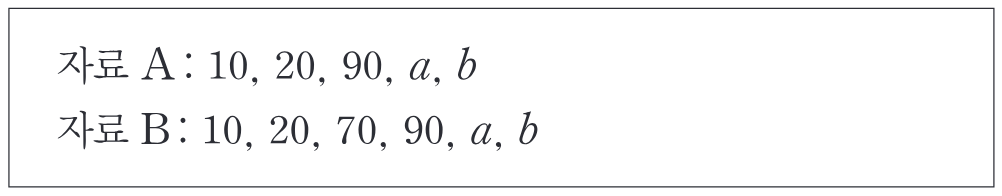
\includegraphics[width=\dmfigw]{figures/fig-0585.png}\end{center}
